\subsection{\F{SMARDDA} modules framework revisited}\label{sec:smagain}
The \F{SMARDDA} modules framework was discussed briefly in the M3.1.2 report~\cite{y2re312},
where particularly its layered structure was noted as relevant to \nep.
Exploration of the literature since, as described in the earlier
\Sec{call1}--\Sec{call8}, has indicated that it is both common and commended
by many workers to construct complex software through aggregation of smaller objects
that may themselves be the basis for physically separate codes. Since the
\F{SMARDDA} software is also built using aggregation in this way, a more
detailed description of this is provided here.

As previously mentioned~\cite{y2re312}, the \F{SMARDDA} software is coded in a
Fortran language style documented in a Culham report~\cite{fprog}
(which is in fact very similar to other styles recommended in the meteorological
community) exemplified by templates which have been posted on github,
as program smardda-qprog~\cite{qprogwebsite}. The new material presented here treats \I{qprog}
as a standalone, independent of the \F{SMARDDA} modules, to emphasise its structure.
Note that the name `qprog' has been deliberately chosen so as not conflict
with other software, the `q' indicating that it poses all the questions to the
developer, since it is purely a skeleton framework accepting nominal inputs
to produce nominal outputs.

Layering is represented by the presence of a
subdirectory LIB, containing a subroutine library compiled from Fortran 
conforming to the older \F{FORTRAN-77} standard. In practice if not in implementation,
the Fortran~95 utility routines which duplicate many of the functions of the
old OLYMPUS library~\cite{y2re312} also share this layer. The most widely used
of these utilities  is log\_m for logging progress made by the code including errors,
and timing information for which modules date\_time\_m and clock\_m are also needed.

There is a script qprog.bash in the repo~\cite{qprogwebsite}
which will set up the files, see \Tab{qprogfiles}, making up a conforming program, and indeed
try to compile, link and run it.
(It does not need \F{SMARDDA} installation if -l for locally complete is set as the first option.)
It is perhaps easiest to start understanding the framework from the documentation of the script.
The program name, its abbreviation (typically one or two letters) and description are defined using
the keys QPROG, Q and STR. The name of a skeleton object module to be tested, its abbreviation
and description are defined using the keys BIGOBJ, BO and BSTR:
\begin{verbatim}
qprog.bash [-l] \
QPROG=xpc Q=xp STR="transport_coefficients" \
BIGOBJ=clcoef BO=cc BSTR="classical_coefficients"
\end{verbatim}
The example is that of a code \I{xpc} to calculate transport coefficients, where
the program name also corresponds to an object, which in this case is the set of
transport models. In the example, for simplicity's sake, only one physical model,
giving the so-called classical or Braginskii coefficients is considered, as object clcoef.
The relation between the objects is shown in \Fig{xpch}. In the example, all objects
are `big', ie. the object description is separated in a file with name ending ``\_h"
from the subroutines which operate on the object in a file with name ending ``\_m",
thus clcoef\_h and clcoef\_m. For a small object, object and associated subroutines
are both combined in one module (``\_m") file. Whereas the full name is used to
describe the namelist QPROGparameters associated with the object 
(namelist is a Fortran language feature for user-friendly keyed
input of values for code variables),
the abbreviation is used to produce type names associated with the object,
notably type Qnumerics (or BOnumerics, xpnumerics and ccnumerics
respectively in the example). The latter separates out the data needed to define
the object, making it possible for instantiation to be deferred (`lazy initialisation').
There is also produced a control module xpcontrol\_m for the program object.

As the templates indicate, each object is largely self-contained within its
module, with subroutines for opening a file which contains input control data, reading from it
and closing it, together with output routines. These latter routines manage files which
might contain numeric dumps of the object variables and descriptions of the
object in plotting formats defined for {\it gnuplot} and {\it ParaView}, to be used in post-processing 
and to visualise aspects of the object in up to 3-D.

The calling tree shown in \Fig{xpc} indicates how the calls, starting with {\tt xpcontrol\_read}
(note the use of the abbreviation in the subroutine name), are arranged so that input data
defining all the objects can be read from a single file.
The $1, 2, 3$ layout is used by the main program xpc~\cite{y2re312}
where in sequence order, $1$~is initialisation, $2$~is compute and $3$~is output and closedown,
but this layout is not generally suitable for use by the other objects.

It is worth noting that there is a .log file
with a special status designed to ensure that as far as possible diagnostics are captured
even should serious errors occur.

It will be seen that, assuming the coefficients of the various transport models combine to
give the total transport by the plasma,  the code will in essence implement the puppeteer
pattern despite the constraint
of a single control file, in that the clcoef\_m  module (and consequently other modules
that might be written to define other sets of coefficients) knows nothing about the \I{xpc} object.
Information needed by clcoef and sibling modules, such as details of the plasma composition, is to be passed
to them in module xpcontrol\_m. The present implementation of this last in xpcontrol\_m
is inelegant, and only adequate for a simple example. For more realistic applications,
understanding and mapping the dependencies between the various inputs will likely
require a graph-based elaboration on the present code design.

Extension to other sibling models such as anomalous transport should be straightforward.
All that has to be arranged is for {\tt xpcontrol\_read} to call {\tt anomcoeff\_readcon},
{\tt xpc\_solve} to call {\tt anomcoeff\_solve} and the various output routines {\tt xpc\_writev},
{\tt xpc\_writeg} and  {\tt xpc\_write} to call their equivalents in the transport coefficient objects.

It is also worth mentioning that use of templates enabled the production of over $1\,400$~lines
of potentially tricky code logic from about $50$~lines of pseudo-code defining variables to be found
in the repo files qprog.txt and clcoef.txt plus
the $2$~lines defining QPROG, Q, etc. above, using a
lengthy but relatively straightforward script, and the total line count allowing
for the utilities is nearly~$4\,000$. In fact the bulk of the remaining code to evaluate classical
transport coefficients to be found on the web-site~\cite{miscwebsite}  was produced with
the help of the reduce-algebra
package~\cite{reducewebsite} which can output mathematical expression in a Fortran syntax.

\begin{table}[h]
\begin{center}
\caption{Files and principal input functions of the QPROG code (xpc example).
The .f90 suffix has been omitted from the filenames.
\label{tab:qprogfiles}}
\begin{tabular}{|p{2.5cm}|p{12.5cm}|}
\hline
File &  Description \\
\hline
QPROG & main program, see its sequence diagram in \Fig{xpc} \\
QPROG\_h & parameters collected in type Qnumerics\_t describing how to construct (at least one) object BIGOBJ
 which is to  be combined with other object data structures such as BIGOBJ\_t into type QPROG\_t \\
QPROG\_m & calls {\tt QPROG\_readcon}, which reads namelist variables 
listed in QPROGparameters and copies them to type Qnumerics\_t variables \\
Qcontrol\_h & data structure of generic top level controls for QPROG (abbreviated as Q) \\
Qcontrol\_m & object of generic top level controls for QPROG (abbreviated as Q), calls {\tt BIGOBJ\_readcon}
 via {\tt Qcontrol\_read} \\
BIGOBJ\_h & data structure of controls for BIGOBJ forming type BOnumerics\_t, also combined type BIGOBJ\_t \\
BIGOBJ\_m & object which reads in object level controls\\
\hline
\end{tabular}
\end{center}
\end{table}


\begin{figure}
\centerline{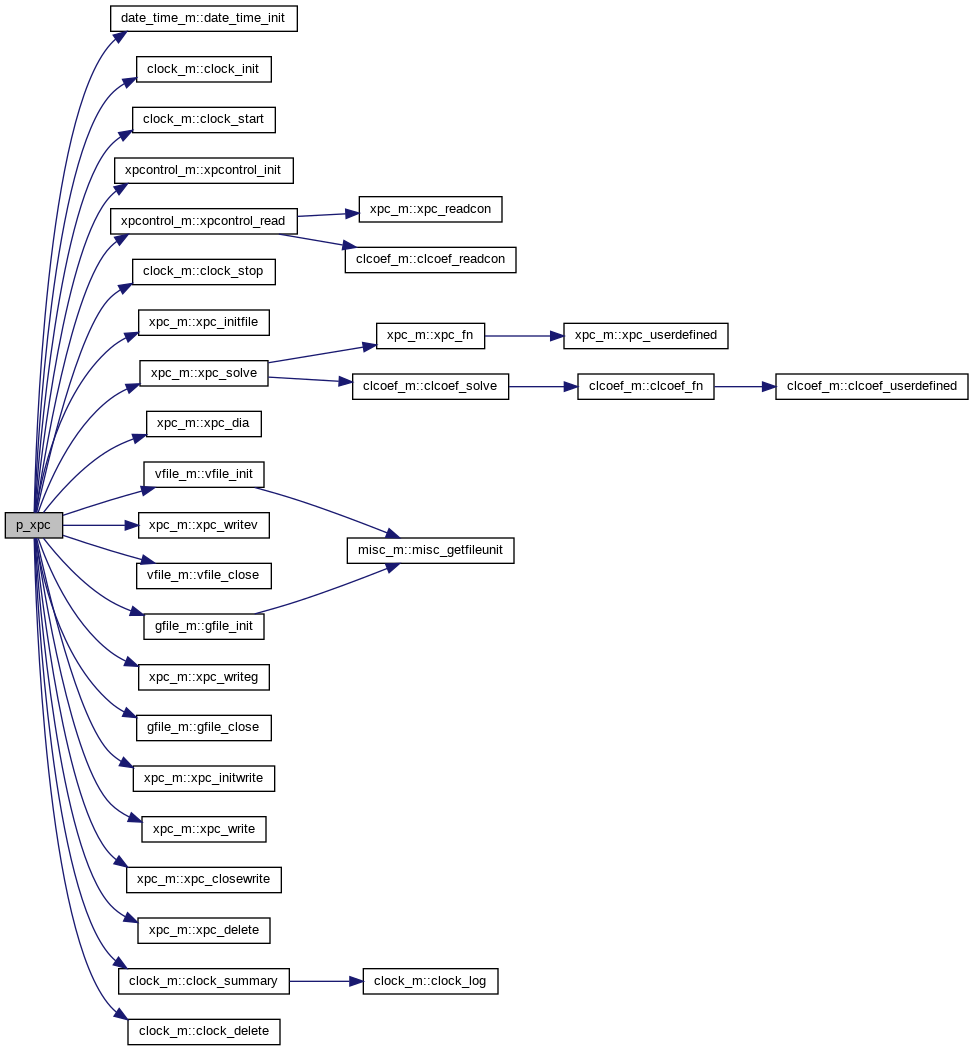
\includegraphics[width=12cm]{../pics/xpc}}
\caption{Calling structure for \F{SMARDDA} style program, plot produced by doxygen
which in this example largely imitates a UML sequence diagram.
The important subroutines to note are {\tt xpcontrol\_read} which coordinates the input of data
defining the two objects clcoef\_t and xpc\_t, and {\tt xpc\_solve} which calls subroutines
operating on both objects to do the work of the code.
(Calls to log\_m subroutines have been suppressed for clarity.)
\label{fig:xpc}}
\end{figure}
\begin{figure}
\centerline{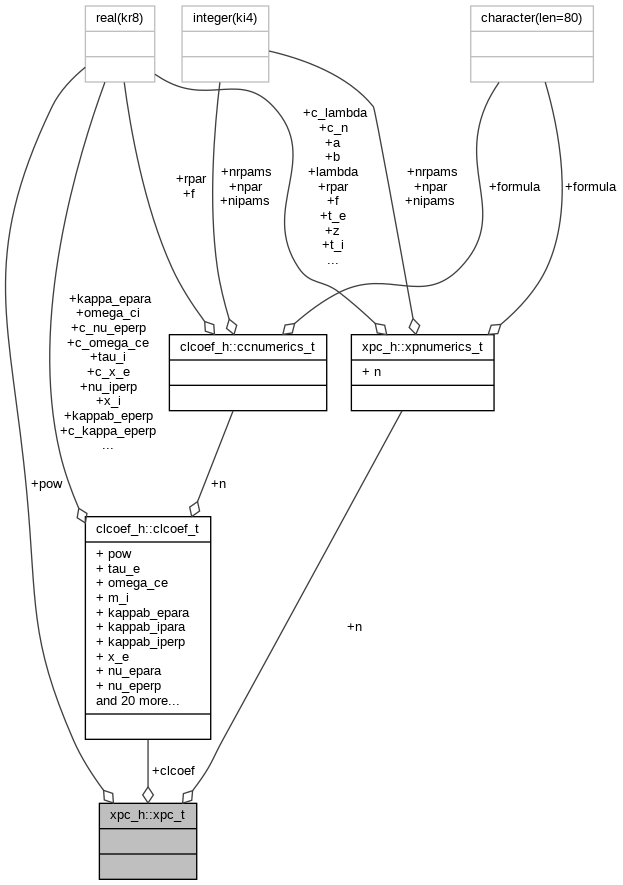
\includegraphics[width=12cm]{../pics/xpch}}
\caption{Data structure for \F{SMARDDA} style program. The plot produced by doxygen
unhelpfully links variables to their simple types (real, integer and character),
however it should be clear each object is associated with a numerics type that
defines how it is to be generated. The figure also indicates how objects are aggregated,
in this instance there is only one object clcoef\_t aggregated with the code level
controls to form the code object xpc\_t.
\label{fig:xpch}}
\end{figure}

\clearpage
%\subsection{DSL-like feature}
%Files input
%qprog.txt contains the input variables that might be used by a range of different objects/modules
%and the default values for these inputs. These variables form part of the top level control QPROG_t
%for the program. A human readable variable for use in
%a namelist will be generated using the first 3 words of the description of each variable.
%In the example, a=... to lambda=... will be copied to QPROG.txt (xpc.txt) and finish in QPROG_h.f90
%bigobj.txt contains the variables defining one object which will normally be defined using the
%instructions resulting from the input variables in qprog.txt, using additional object level controls
%(and of course code to be written by the user).
%In the example, tau_e... and c_tau_e... will be copied to BIGOBJ.txt (clcoef.txt)
%and finish in BIGOBJ_h.f90.
%makefile.QPROG makefile to compile and link QPROG 
%QPROG\_case0.ctl & input file for QPROG containing complete list of namelists
%
%Outputs from execution of QPROG
%xpc\_case0.log log data such as date and time of run, cpu measured by internal clocks
%xpc\_case0\_xpc.out indicative output, precisely object level controls for BIGOBJ
